
%%% Local Variables: 
%%% mode: latex
%%% TeX-master: t
%%% End: 

\documentclass{article}
\usepackage{graphicx}
\begin{document}
Vinay Jayaram and Lukas Sonnenberg\\
Task 3

\section{Figure 1}
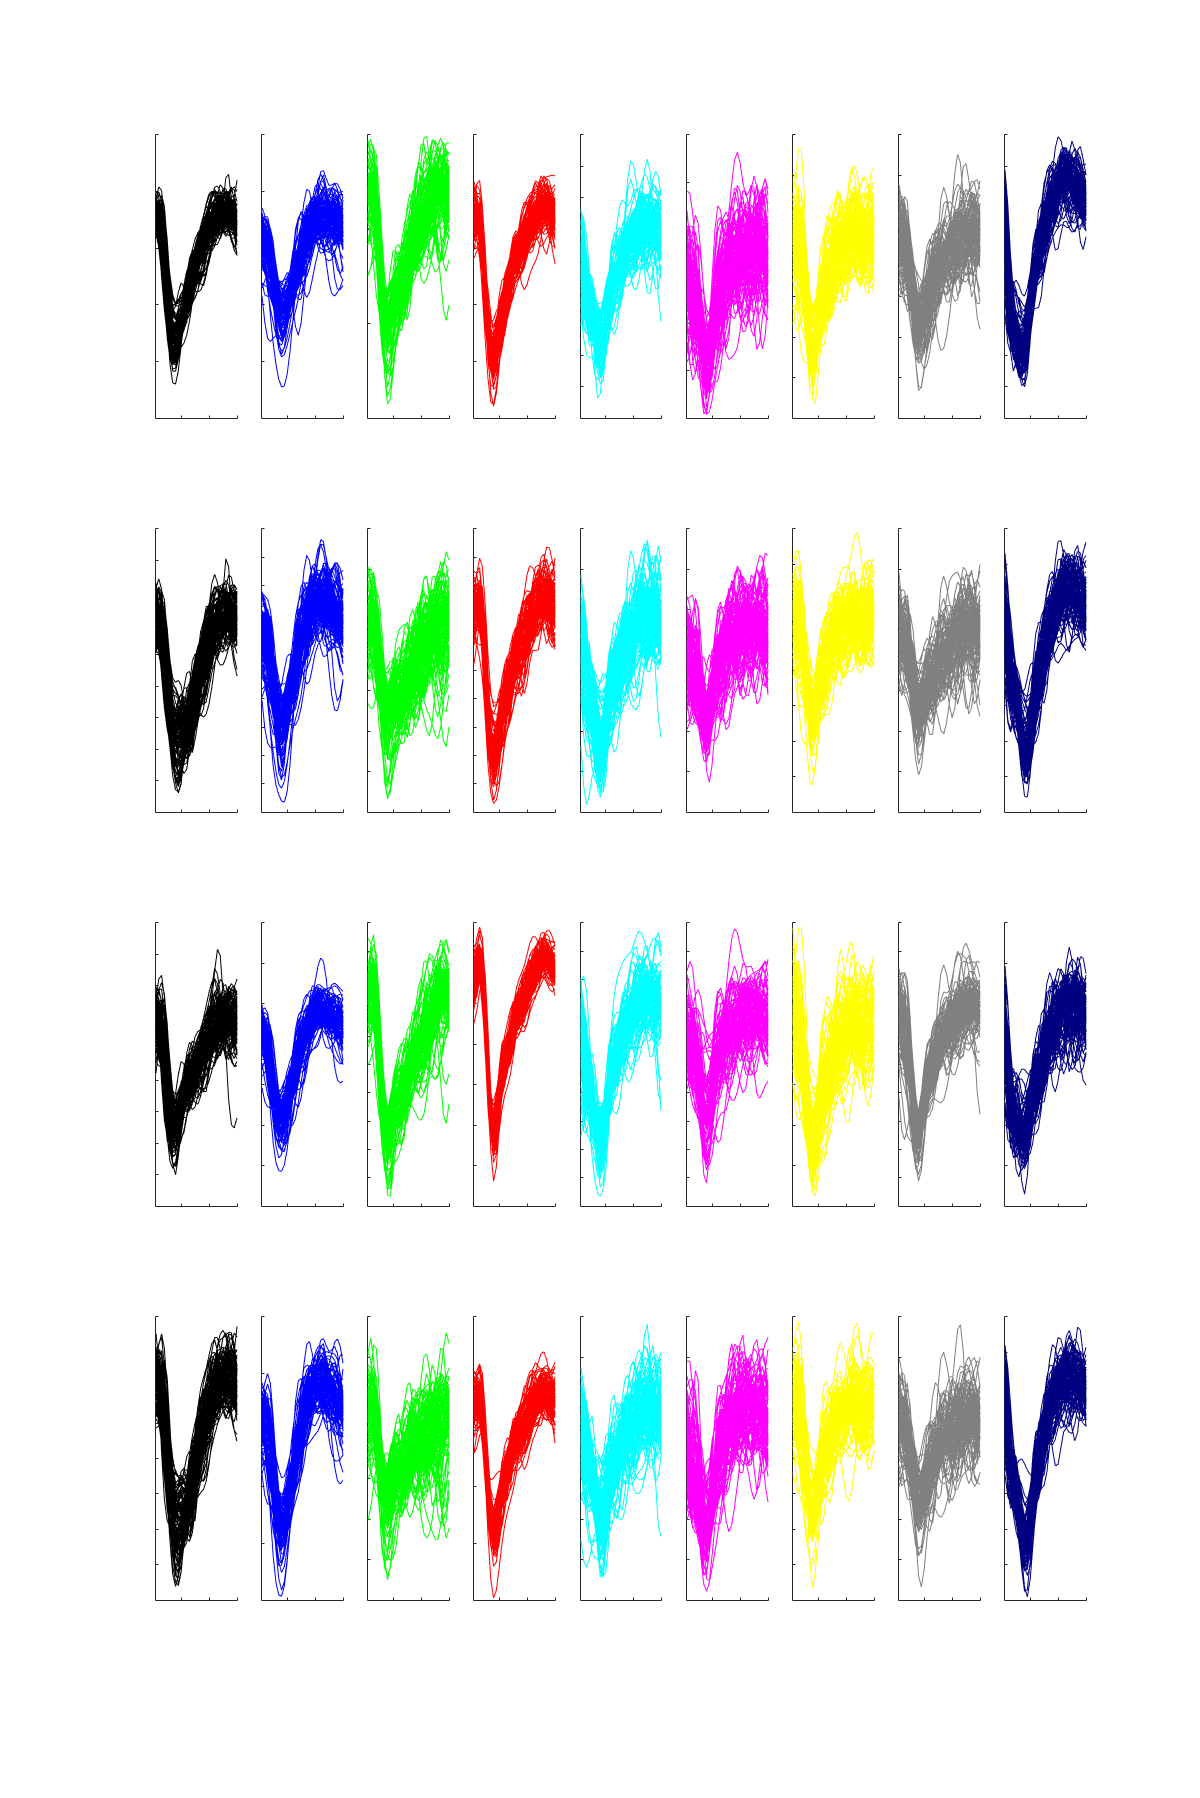
\includegraphics[width=\textwidth]{Figure1.png}

\section{Figure 2}
\includegraphics[width=\textwidth]{Figure2.png}
\section{Figure 3}
\includegraphics[width=\textwidth]{Figure3.png}

Considering all the visualizations I would say that black and dark blue are the same unit, but the rest are single units. 

It is unclear why the png's aren't coming out right...sorry. The PNGs themselves are fine. 
\end{document}
